%%%%%%%%%%%%%%%%%%%%%%%%%%%%%%%%%%%%%%%%%
% Beamer Presentation
% LaTeX Template
% Version 1.0 (10/11/12)
%
% This template has been downloaded from:
% http://www.LaTeXTemplates.com
%
% License:
% CC BY-NC-SA 3.0 (http://creativecommons.org/licenses/by-nc-sa/3.0/)
%
%%%%%%%%%%%%%%%%%%%%%%%%%%%%%%%%%%%%%%%%%

%----------------------------------------------------------------------------------------
%	PACKAGES AND THEMES
%----------------------------------------------------------------------------------------

\documentclass[UTF8,aspectratio=169,12pt]{ctexbeamer}

\usepackage{hyperref}
\hypersetup{
	colorlinks=true,
	linkcolor=red,
	anchorcolor=blue,
	citecolor=green
}

\mode<presentation> {
	
	% The Beamer class comes with a number of default slide themes
	% which change the colors and layouts of slides. Below this is a list
	% of all the themes, uncomment each in turn to see what they look like.
	
	%\usetheme{default}
	%\usetheme{AnnArbor}
	%\usetheme{Antibes}
	%\usetheme{Bergen}
	%\usetheme{Berkeley}
	%\usetheme{Berlin}
	%\usetheme{Boadilla}
	%\usetheme{CambridgeUS}
	%\usetheme{Copenhagen}
	%\usetheme{Darmstadt}
	%\usetheme{Dresden}
	%\usetheme{Frankfurt}
	%\usetheme{Goettingen}
	%\usetheme{Hannover}
	%\usetheme{Ilmenau}
	%\usetheme{JuanLesPins}
	%\usetheme{Luebeck}
	\usetheme{Madrid}
	%\usetheme{Malmoe}
	%\usetheme{Marburg}
	%\usetheme{Montpellier}
	%\usetheme{PaloAlto}
	%\usetheme{Pittsburgh}
	%\usetheme{Rochester}
	%\usetheme{Singapore}
	%\usetheme{Szeged}
	%\usetheme{Warsaw}
	
	% As well as themes, the Beamer class has a number of color themes
	% for any slide theme. Uncomment each of these in turn to see how it
	% changes the colors of your current slide theme.
	
	%\usecolortheme{albatross}
	%\usecolortheme{beaver}
	%\usecolortheme{beetle}
	%\usecolortheme{crane}
	%\usecolortheme{dolphin}
	%\usecolortheme{dove}
	%\usecolortheme{fly}
	%\usecolortheme{lily}
	%\usecolortheme{orchid}
	%\usecolortheme{rose}
	%\usecolortheme{seagull}
	%\usecolortheme{seahorse}
	%\usecolortheme{whale}
	%\usecolortheme{wolverine}
	
	%\setbeamertemplate{footline} % To remove the footer line in all slides uncomment this line
	%\setbeamertemplate{footline}[page number] % To replace the footer line in all slides with a simple slide count uncomment this line
	
	%\setbeamertemplate{navigation symbols}{} % To remove the navigation symbols from the bottom of all slides uncomment this line
}

\usepackage{graphicx} % Allows including images
\graphicspath{{./figs/}}
\usepackage{booktabs} % Allows the use of \toprule, \midrule and \bottomrule in tables
\usepackage{longtable}
\usepackage{xcolor}
\usepackage{minted}
\usepackage{listings}
\lstset{numbers=left, %设置行号位置
	numberstyle=\tiny, %设置行号大小
	keywordstyle=\color{blue}, %设置关键字颜色
	commentstyle=\color[cmyk]{1,0,1,0}, %设置注释颜色
	frame=single, %设置边框格式
	escapeinside=``, %逃逸字符(1左面的键),用于显示中文
	%breaklines, %自动折行
	extendedchars=false, %解决代码跨页时,章节标题,页眉等汉字不显示的问题
	xleftmargin=2em,xrightmargin=2em, aboveskip=1em, %设置边距
	tabsize=4, %设置tab空格数
	showspaces=false %不显示空格
}
% Fonts
% \usepackage{libertine}
% \setmonofont{Courier}
%\setCJKsansfont[ItalicFont=Noto Serif CJK SC Black, BoldFont=Noto Sans CJK SC Black]{Noto Sans CJK SC}

%\def\imagepath{./resources/graphics}
%\usepackage[imagepath=\imagepath]{ditaa}
%\graphicspath{ {\imagepath/} }


%\usepackage{pgfpages}
%\setbeameroption{show notes on second screen}
%%----------------------------------------------------------------------------------------
%	TITLE PAGE
%----------------------------------------------------------------------------------------

\title[第8讲]{第8讲 :全局页替换算法} % The short title appears at the bottom of every slide, the full title is only on the title page
\subtitle{第六节:面向缓存的页替换算法 -- LRU-K \& 2Q}
\author{向勇、陈渝、李国良} % Your name
\institute[清华大学] % Your institution as it will appear on the bottom of every slide, may be shorthand to save space
{
	清华大学计算机系 \\ % Your institution for the title page
	\medskip
	\textit{xyong,yuchen,liguoliang@tsinghua.edu.cn} % Your email address
}
\date{\today} % Date, can be changed to a custom date


\begin{document}

\begin{frame}
\titlepage % Print the title page as the first slide
\end{frame}

%\begin{frame}
%\frametitle{提纲} % Table of contents slide, comment this block out to remove it
%\tableofcontents % Throughout your presentation, if you choose to use \section{} and \subsection{} commands, these will automatically be printed on this slide as an overview of your presentation
%\end{frame}
%
%%----------------------------------------------------------------------------------------
%%	PRESENTATION SLIDES
%%----------------------------------------------------------------------------------------

%----------------------------------------------
\begin{frame}[plain]
	\frametitle{LRU-K}
	\begin{columns}
		\begin{column}{.1\textwidth}
			\centering
%			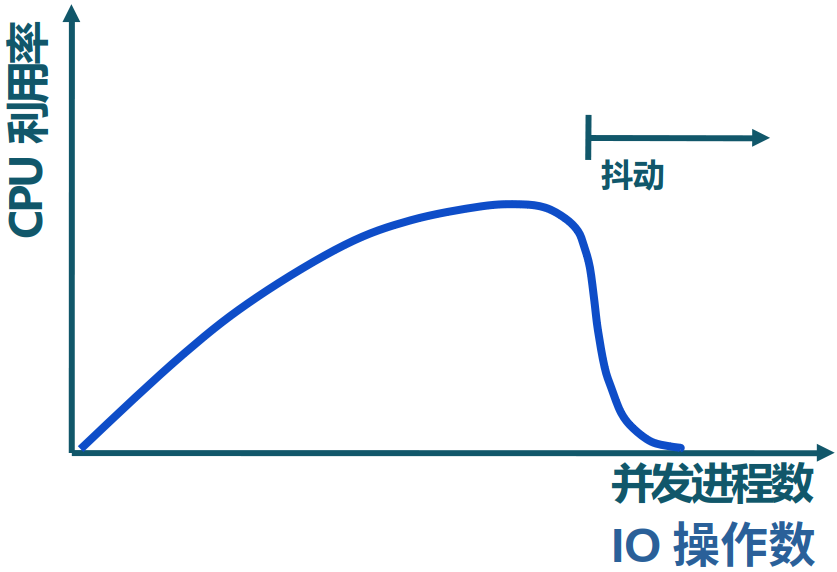
\includegraphics[width=.6\textwidth]{mem-trash}
			%			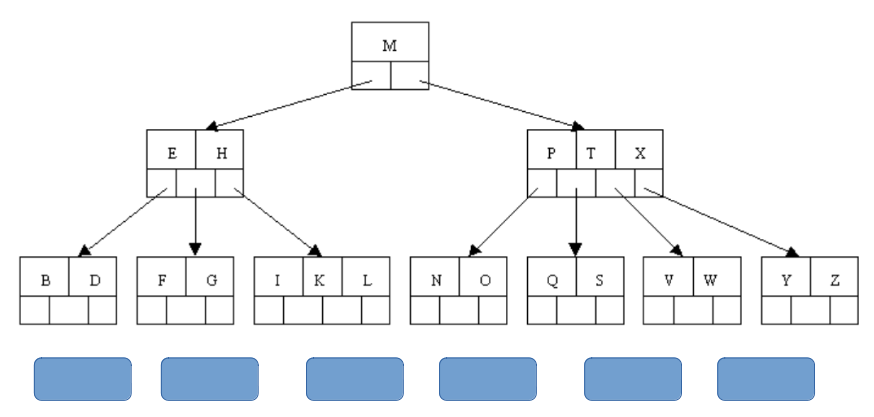
\includegraphics[width=1.2\textwidth]{btree}
		\end{column}
		
		\begin{column}{.9\textwidth}
			
			\begin{itemize}
				\item 有更简洁的LRU+LFU的设计思路吗? 能够应对:
				\begin{itemize}
					
					\item 顺序访问:所有的块一个接一个被访问,不存在重访问
					\item 循环访问:所有块都按照一定的间隔重复访问
					\item 时间密集访问:最近被访问的块是将来最有可能被访问的
					\item 概率访问:所有块都有固定的访问概率,所有块都互相独立地根据概率被访问
					
					
				\end{itemize}
			\end{itemize}
		\centering
			最近使用过K次?
			
		\end{column}
		
		
	\end{columns}
\end{frame}



%----------------------------------------------
\begin{frame}[plain]
	\frametitle{LRU-K}
	\begin{columns}
		\begin{column}{.4\textwidth}
			\centering
			%			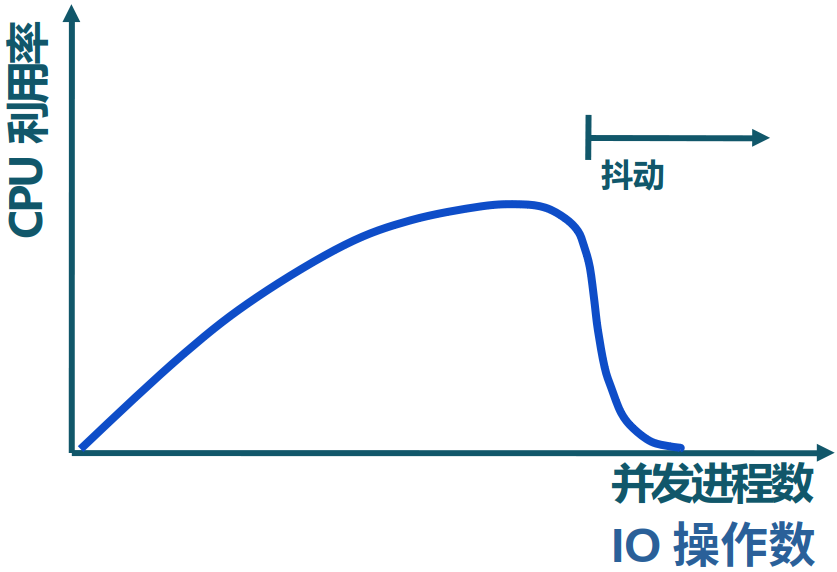
\includegraphics[width=.6\textwidth]{mem-trash}
			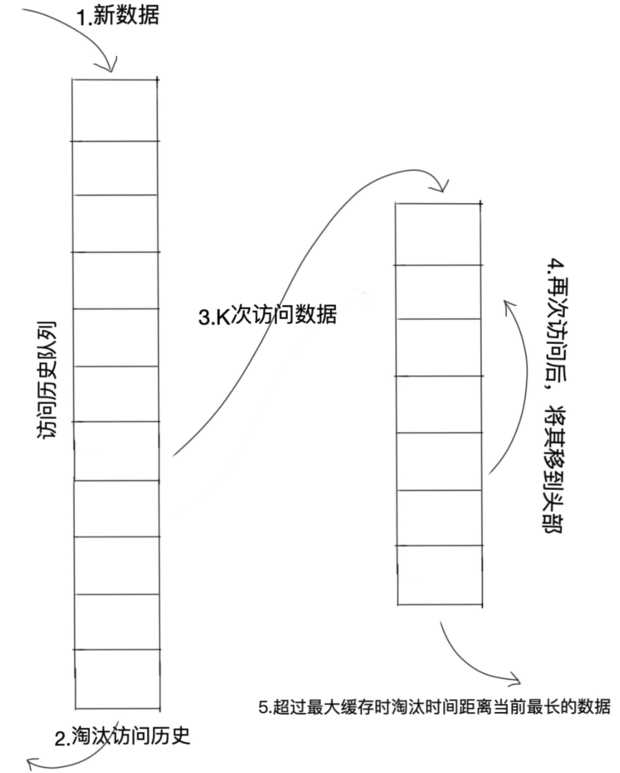
\includegraphics[width=1.\textwidth]{lru-k}
		\end{column}
		
		\begin{column}{.6\textwidth}
			
			% \begin{itemize}
				% \item LRU-K
				\begin{itemize}
					
					\item LRU-K是基于LRU算法的扩展,其中K代表最近访问的次数,从某种意义上,LRU可以看作是LRU-1算法,引入K的意义是为了解决缓存污染问题。
					\item 其核心理念是从“数据最近被访问过1次”蜕变成“数据最近被访问过K次,那么将来被访问的概率会更高”。
					
					
				\end{itemize}
			% \end{itemize}
			
			
		\end{column}
		
		
	\end{columns}
\end{frame}


%----------------------------------------------
\begin{frame}[plain]
	\frametitle{LRU-K}
	\begin{columns}
		\begin{column}{.4\textwidth}
			\centering
			%			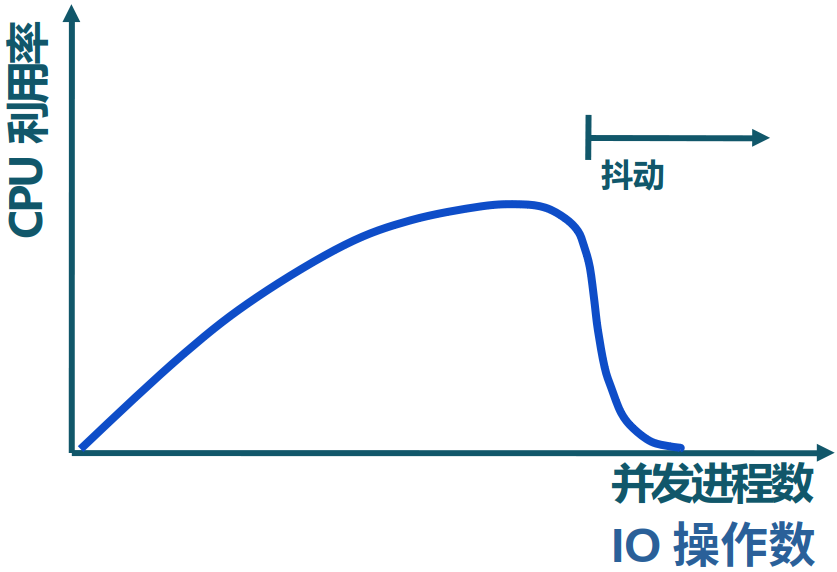
\includegraphics[width=.6\textwidth]{mem-trash}
			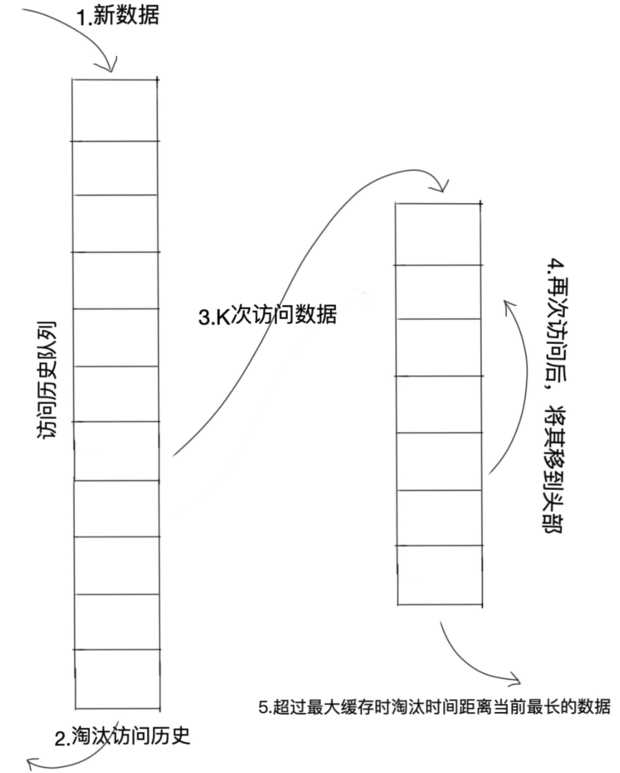
\includegraphics[width=1.\textwidth]{lru-k}
		\end{column}
		
		\begin{column}{.6\textwidth}
			
			%\begin{itemize}
			%	\item LRU-K
				\begin{itemize}
					
					\item LRU-K与LRU区别:LRU-K多了一个数据访问历史记录队列(需要注意的是,访问历史记录队列并不是缓存队列,所以是不保存数据本身的,只是保存对数据的访问记录),访问历史记录队列中维护着数据被访问的次数以及时间戳。
					\item 只有当这个数据被访问的次数大于等于K值时,才会从历史记录队列中删除,然后把数据加入到缓存队列中去。
					
				\end{itemize}
			% \end{itemize}
			
			
		\end{column}
		
		
	\end{columns}
\end{frame}

%----------------------------------------------
\begin{frame}[plain]
	\frametitle{LRU-K}
	\begin{columns}
		\begin{column}{.4\textwidth}
			\centering
			%			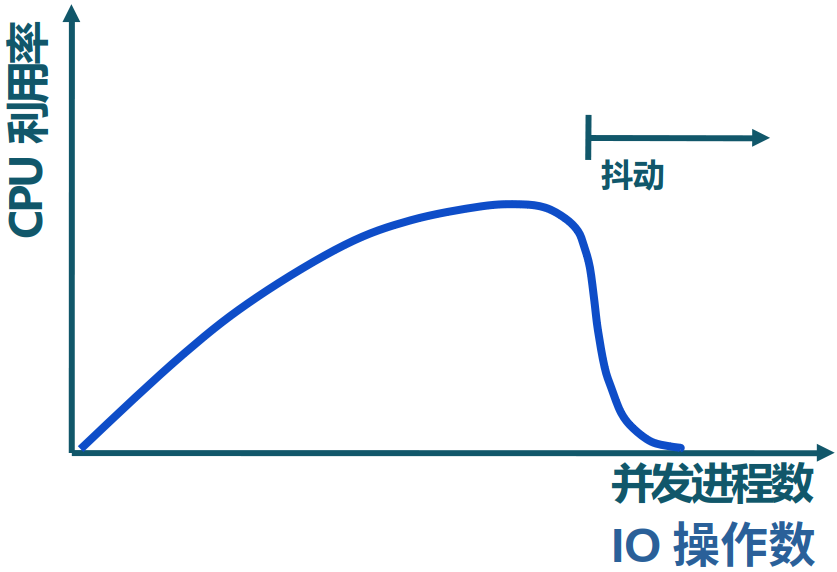
\includegraphics[width=.6\textwidth]{mem-trash}
						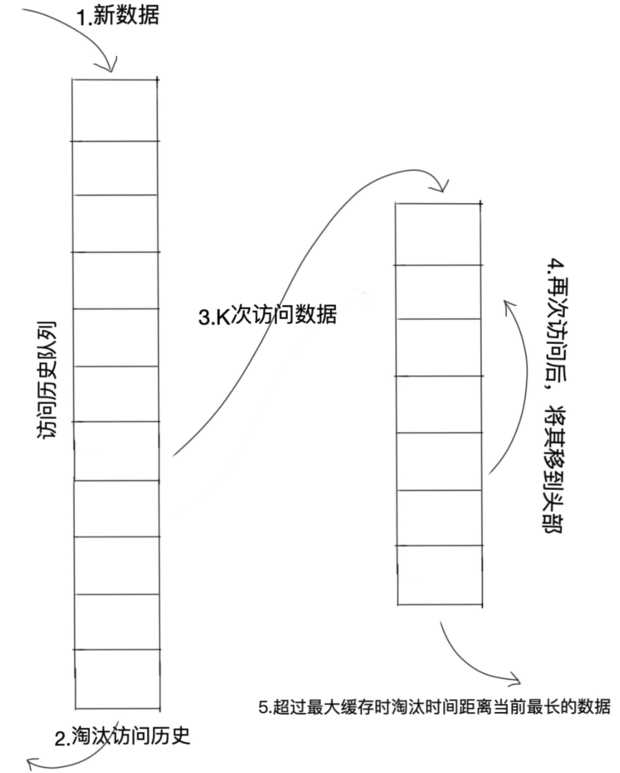
\includegraphics[width=1.\textwidth]{lru-k}
		\end{column}
		
		\begin{column}{.6\textwidth}
			
			%\begin{itemize}
			%	\item LRU-K
				\begin{itemize}
					
					\item 数据第一次被访问时,加入到历史访问记录队列中,访问次数为1,初始化访问时间戳;
					\item 如果数据访问次数没有达到K次,则访问次数+1,更新时间戳。当队列满了时,按照某种规则(LRU或者FIFO)将历史记录淘汰;%为了避免历史数据污染未来数据的问题,还需要加上一个有效期限,对超过有效期的访问记录,进行重新计数;
					\item 当访问历史队列中的数据访问次数达到K次后,将数据索引从历史队列删除,将数据移到缓存队列中,缓存队列重新按照时间排序;
					\item 缓存数据队列中被再次访问后,重新排序
					\item 需要淘汰数据时,淘汰缓存队列中排在末尾的数据,即:淘汰“倒数第K次访问离现在最久”的数据
					
					
				\end{itemize}
			%\end{itemize}

			
		\end{column}
		
		
	\end{columns}
\end{frame}


%----------------------------------------------
\begin{frame}[plain]
	\frametitle{评价LRU-K}
	\begin{columns}
		\begin{column}{.4\textwidth}
			\centering
			%			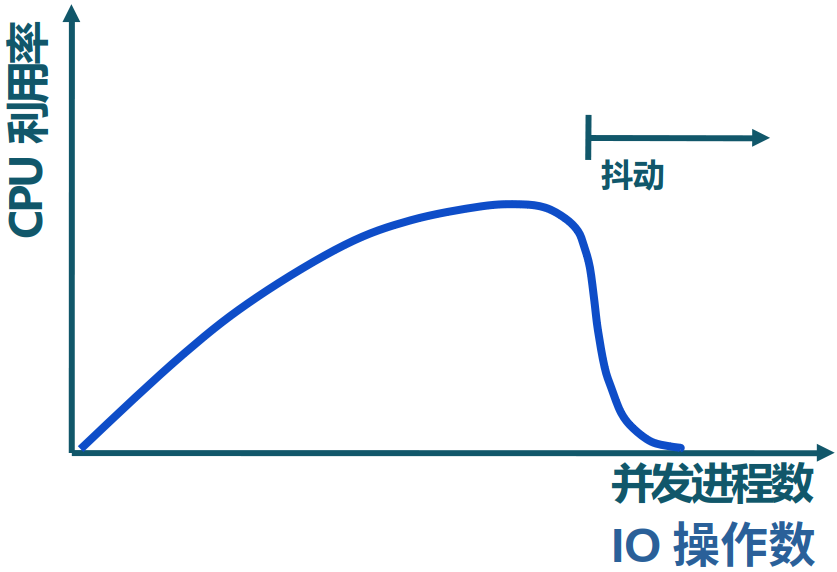
\includegraphics[width=.6\textwidth]{mem-trash}
			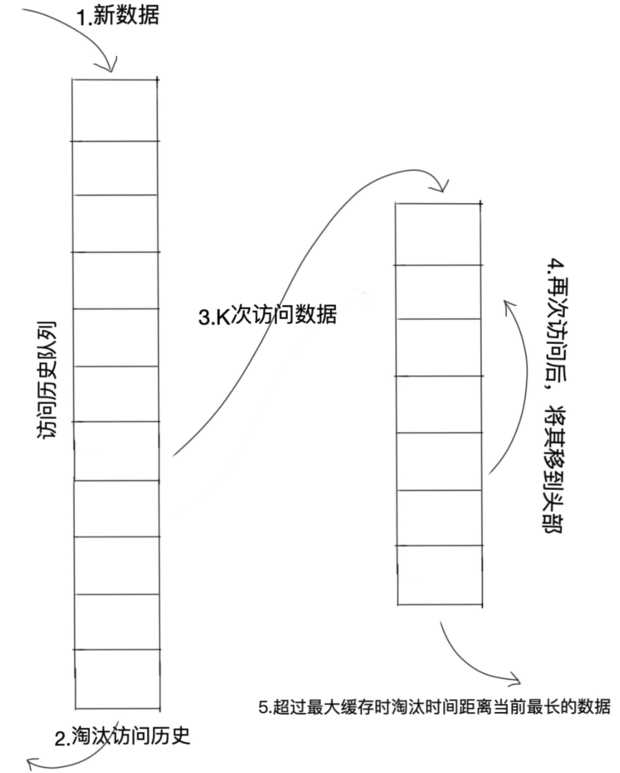
\includegraphics[width=1.\textwidth]{lru-k}
		\end{column}
		
		\begin{column}{.6\textwidth}
			
			%\begin{itemize}
			%	\item 评价 LRU-K 
				\begin{itemize}
					
					\item LRU-K降低了“缓存污染”带来的问题,命中率比LRU要高。
					\item 在实际应用中,LRU-2是综合各种因素后最优的选择。
					\item LRU-3或更大的K值命中率会高,但适应性差,一旦访问模式发生变化,需要大量的新数据访问才能将历史热点访问记录清除掉。
					\item LRU-K数据缓存队列一般是一个优先级队列。排序操作需要额外的O(logN)的时间复杂度,N为数据缓存队列的大小。
					
				\end{itemize}
			%\end{itemize}
			\centering
			\large 从能否进一步改进?
		\end{column}
		
		
	\end{columns}
\end{frame}




%----------------------------------------------
\begin{frame}[plain]
	\frametitle{2Q}
	\begin{columns}
		\begin{column}{.4\textwidth}
			\centering
			%			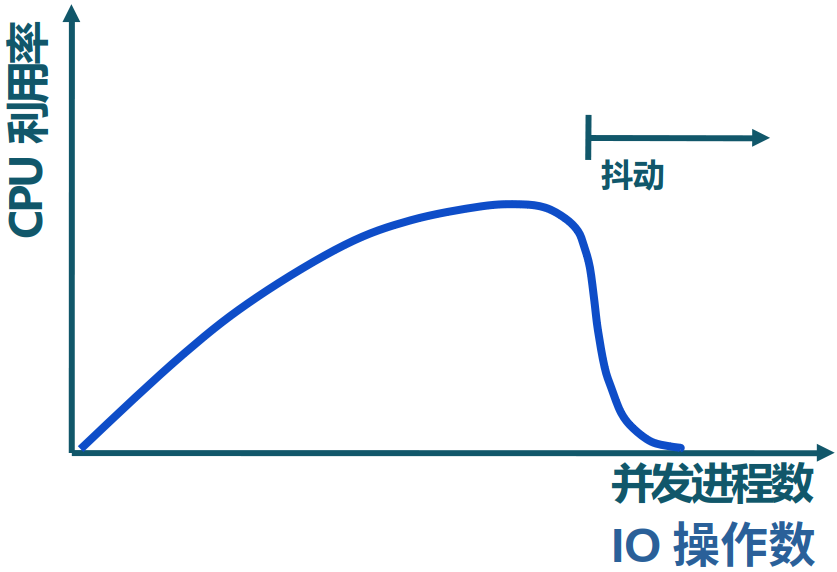
\includegraphics[width=.6\textwidth]{mem-trash}
			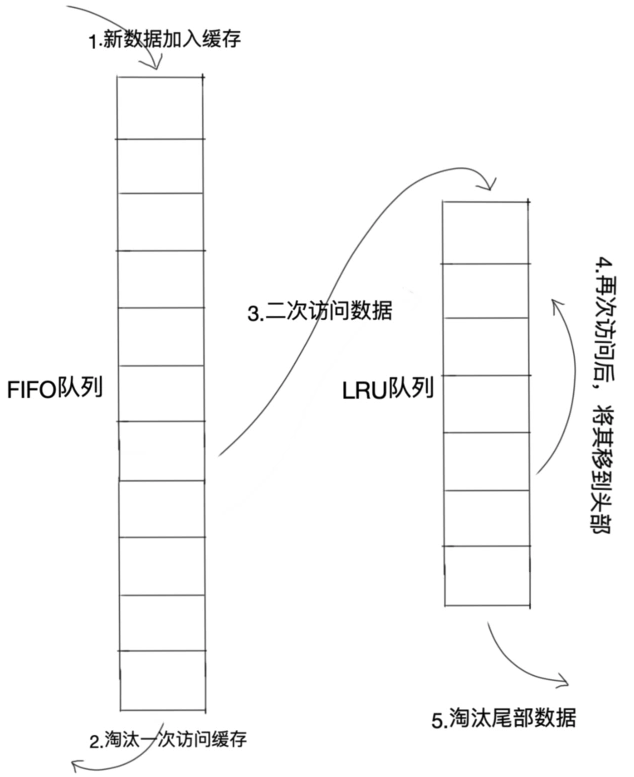
\includegraphics[width=1.\textwidth]{2q}
		\end{column}
		
		\begin{column}{.6\textwidth}
			
			%\begin{itemize}
			%	\item 2Q
				\begin{itemize}
					
					\item 2Q算法类似于LRU-2,不同点在于2Q将LRU-2算法中的访问历史队列(注意这不是缓存数据的)改为一个FIFO缓存队列,即:2Q算法有两个缓存队列,一个是FIFO队列(First in First out,先进先出),一个是LRU队列。
					\item 当数据第一次访问时,2Q算法将数据缓存在FIFO队列里面,当数据第二次被访问时,则将数据从FIFO队列移到LRU队列里面,两个队列各自按照自己的方法淘汰数据。
				\end{itemize}
			%\end{itemize}
%			\centering
%			\large 从能否进一步改进?
		\end{column}
		
		
	\end{columns}
\end{frame}


%----------------------------------------------
\begin{frame}[plain]
	\frametitle{2Q}
	\begin{columns}
		\begin{column}{.4\textwidth}
			\centering
			%			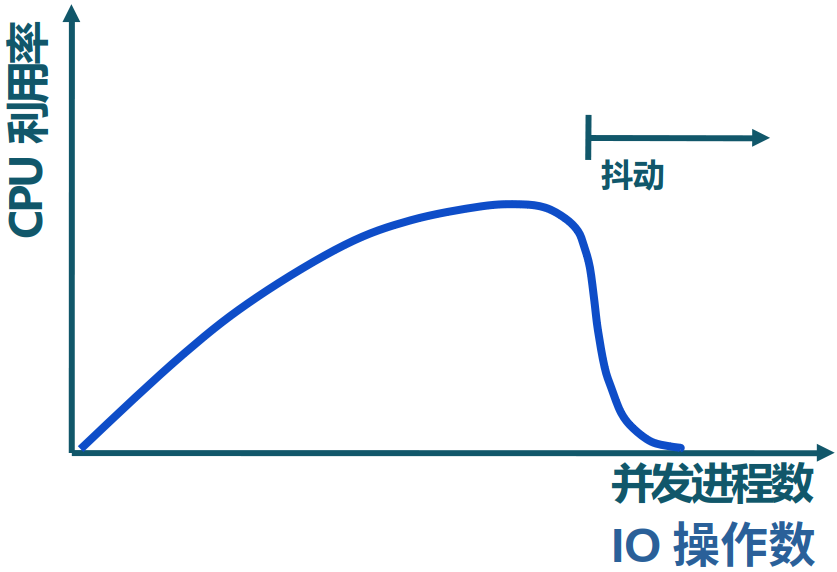
\includegraphics[width=.6\textwidth]{mem-trash}
			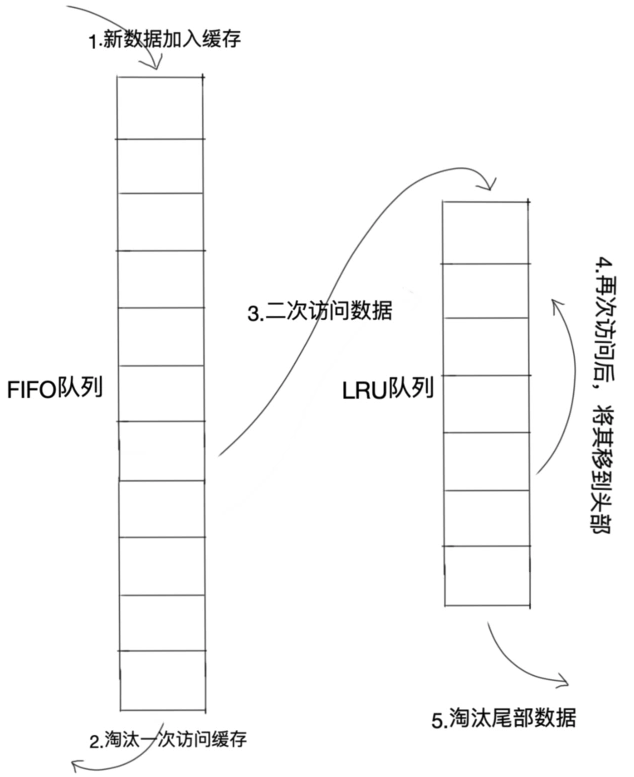
\includegraphics[width=1.\textwidth]{2q}
		\end{column}
		
		\begin{column}{.6\textwidth}
			
			%\begin{itemize}
			%	\item 2Q
				\begin{itemize}
					
					\item 新访问的数据先插入到FIFO队列中;
					\item 如果数据在FIFO队列中一直没有被再次访问,则最终按照FIFO规则淘汰;
					\item 如果数据在FIFO队列中被再次访问,则将数据从FIFO删除,加入到LRU队列头部;
					\item 如果数据在LRU队列再次被访问,则将数据移到LRU队列头部;
					\item LRU队列淘汰末尾的数据。
				\end{itemize}
			%\end{itemize}

		\end{column}
		
		
	\end{columns}
\end{frame}



%----------------------------------------------
\begin{frame}[plain]
	\frametitle{评价2Q}
	\begin{columns}
		\begin{column}{.4\textwidth}
			\centering
			%			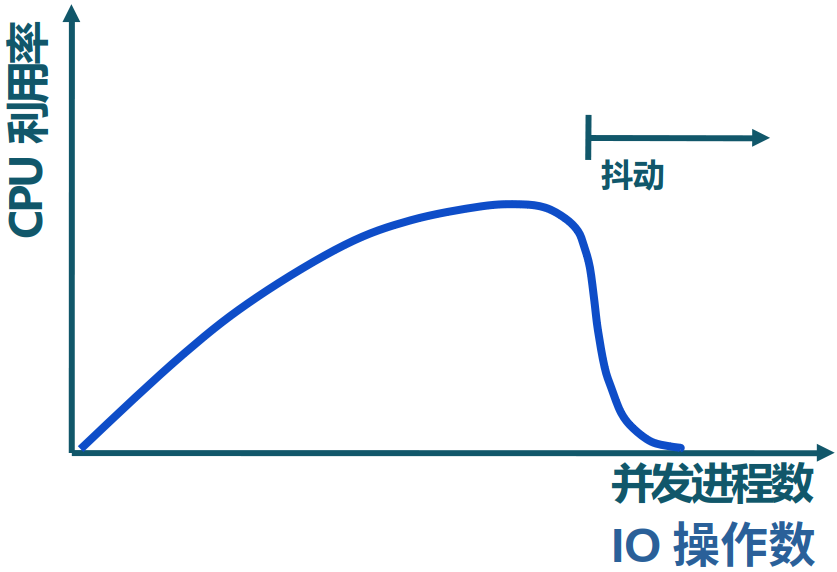
\includegraphics[width=.6\textwidth]{mem-trash}
			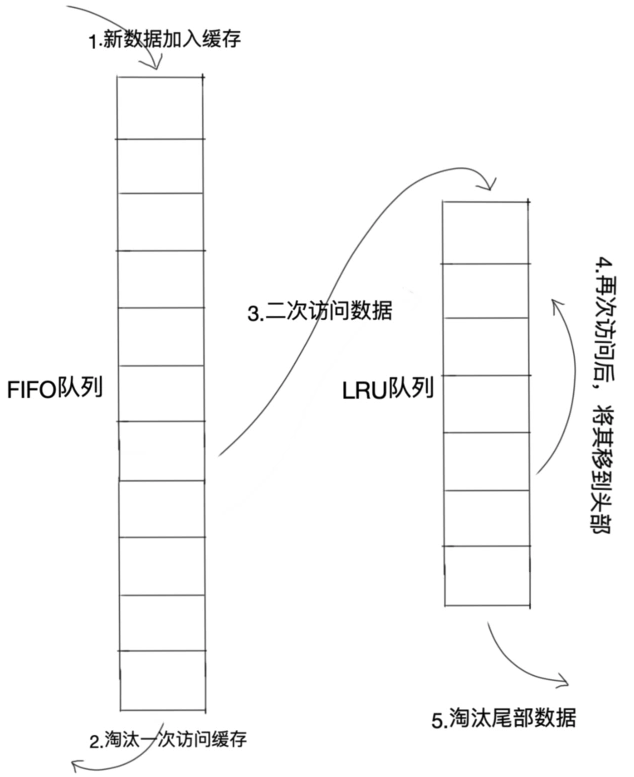
\includegraphics[width=1.\textwidth]{2q}
		\end{column}
		
		\begin{column}{.6\textwidth}
			
			%\begin{itemize}
			%	\item 评价2Q
				\begin{itemize}
					\item 计算开销小于LRU-2
					\item 命中率与LRU-2类似,命中率要高于LRU
					\item 需要维护两个队列,代价是FIFO和LRU代价之和
					\item 仍然需要配置参数

				\end{itemize}
			%\end{itemize}
						\centering
						\large 从能否进一步改进?
												
		\end{column}
		
		
	\end{columns}
\end{frame}


%----------------------------------------------------------------------------------------

\end{document}
